%&LaTeX

\chapter{Overview}
Nalu constructs a linear system by mapping degrees of freedom at mesh nodes
to equations, i.e., rows in the matrix and rhs vector. In a parallel run,
the linear system that is given to the solver contains equations that
correspond to locally owned mesh nodes, which are the mesh nodes that are
owned by the local MPI rank. Each MPI rank can also have mesh nodes which
are shared but not owned, as well as mesh nodes that are ghosted.
 Shared-but-not-owned nodes are owned by another MPI rank but are
connected to an element that is locally owned. Ghosted mesh nodes tend to
arise in cases that involve periodic boundaries, and cases that involve
mesh contact which is handled via a Discontinuous Galerkin scheme.

Consider the simple two-element
mesh decomposed onto 2 MPI ranks and shown in figures \ref{decomp1} and
\ref{locallyowned}.

\begin{figure}[ht]
\centering
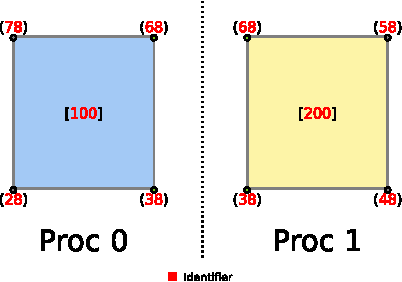
\includegraphics{figures/stkMeshUniversalPart.pdf}
\caption{Parallel-decomposed mesh. Two elements, one on each MPI processor.
Note that some mesh nodes appear on both processors.}
\label{decomp1}
\end{figure}

\begin{figure}[ht]
\centering
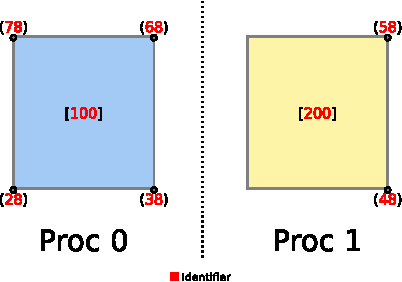
\includegraphics{figures/stkMeshLocallyOwnedPart.pdf}
\caption{Locally-owned nodes.  Nodes 38 and 68 are owned by process 0 and are 
shared but not owned by process 1.}
\label{locallyowned}
\end{figure}

Nalu uses Tpetra::Map objects to identify the degrees of freedom and processor layout.
There are two maps, \code{ownedRowsMap\_} and \code{sharedNotOwnedRowsMap\_}.
For the simple two-element mesh in this example, figure \ref{maps1}
shows how the owned and shared maps would be defined.

\begin{figure}[ht]
\centering
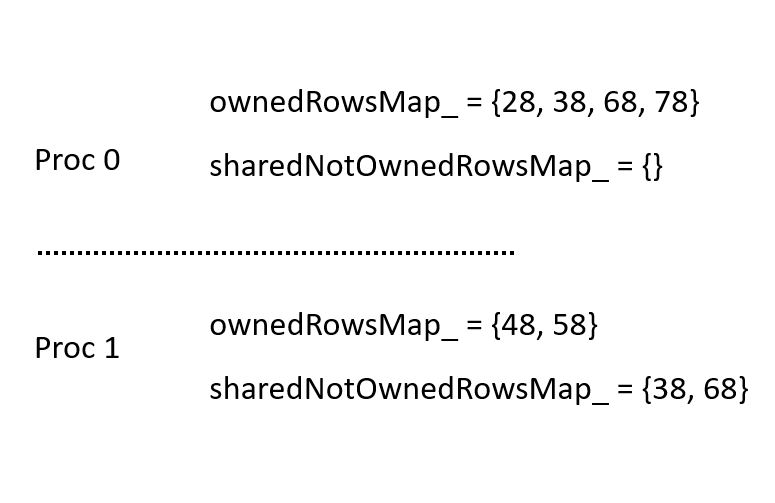
\includegraphics[scale=0.7]{figures/maps1.jpg}
\caption{Owned and Shared-not-Owned Maps.}
\label{maps1}
\end{figure}

We then create \code{Tpetra::CrsGraph} objects for owned and shared
(these objects are called
\code{ownedGraph\_} and \code{sharedNotOwnedGraph\_}), each using the appropriate
row-map. These graphs both use the same column map, and the creation and
initialization of the column map will be discussed in a later section.
We also create Tpetra::CrsMatrix objects for owned and shared, called
\code{ownedMatrix\_} and \code{sharedNotOwnedMatrix\_}.

Each processor contributes an element-matrix of coefficients for its local
elements as shown in figure \ref{elemContribs1}.

\begin{figure}[ht]
\centering
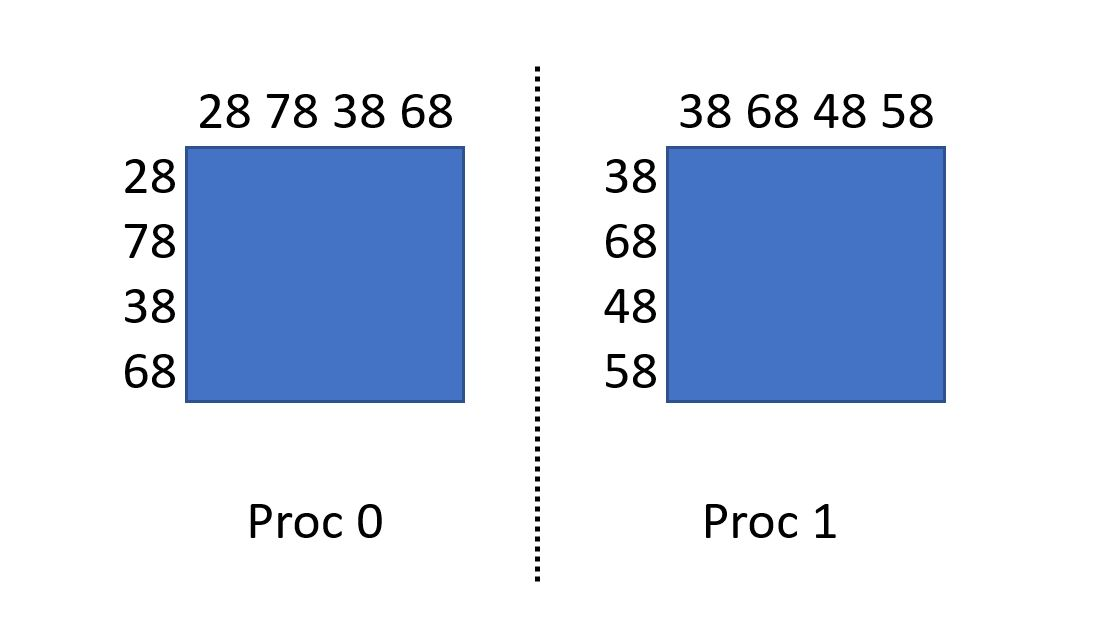
\includegraphics[scale=0.5]{figures/elemContribs.jpg}
\caption{Element-matrix contributions per processor.}
\label{elemContribs1}
\end{figure}

Note that processor 1 has contributions for some rows (38 and 68) that it doesn't
own. Each processor contributes the rows of its element-contributions to
the appropriate matrix object depending on whether the row is owned or not.
Once all element-contributions have been assembled, the contents of the
shared-but-not-owned matrix are sent to the appropriate processors and added
to the owned matrix.
\begin{lstlisting}[caption={Assembly using export}, label=doexport]
  sharedNotOwnedMatrix_->fillComplete();

  ownedMatrix_->doExport(*sharedNotOwnedMatrix_,
                         *exporter_, Tpetra::ADD);

  ownedMatrix_->fillComplete();
\end{lstlisting}
This is done using Tpetra methods as shown in
listing \ref{doexport}. The result is an assembled global matrix as shown
in figure \ref{assembled}.

\begin{figure}[ht]
\centering
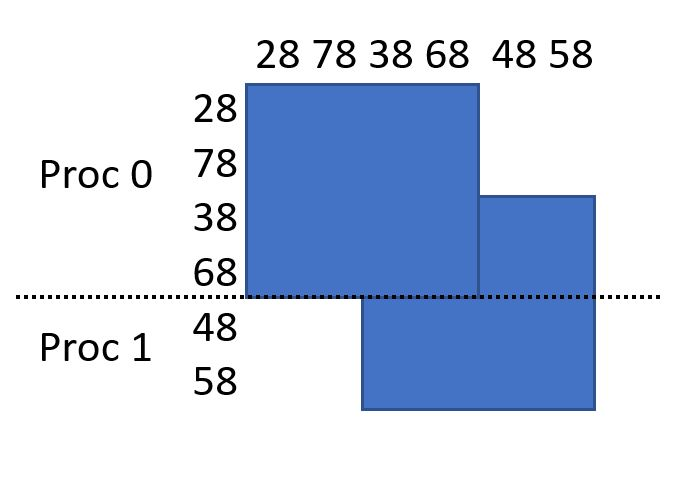
\includegraphics[scale=0.5]{figures/assembled.jpg}
\caption{Assembled \code{ownedMatrix\_}.}
\label{assembled}
\end{figure}

Note that corresponding operations are performed in the assembly of the
right-hand-side vector, in terms of owned and shared, export, etc.

Once the \code{fillComplete} operation has completed, the linear system is
fully assembled and is ready to be passed to solvers and/or preconditioners.
Later sections will go into more detail on the construction of the
column map and graph objects, in order to correctly and efficiently
incorporate off-processor column entries, etc.

We broadly split the construction of the linear system into two
phases called initialization and assembly. The initialization phase
is where we construct the maps, perform communication to send column
indices to appropriate processors, and construct graph objects.
The assembly phase is where we assemble coefficient values into the
matrix using a ``sum-into'' operation, and also modify the linear
system to enforce boundary conditions. In simulations where the structure
of the linear system doesn't change from one timestep to the next, we
can gain efficiency by performing the initialization phase once and
then reusing the data structures for many assembly and solve phases.

Mesh nodes can also be ghosted, which means they are copied from the owning
processor to another processor which has no connectivity relationship with
those nodes. Ghosted nodes (on the receiving processor) are neither owned
nor shared. Ghosting can happen when periodic boundaries of the mesh are mapped
to each other across MPI processors. Ghosting can also happen when a mesh
surface is in contact with another mesh surface where the elements on either
side of the contact don't share connected nodes. See figure \ref{slidingmesh1}
for an example of a mesh with contact boundaries going through the middle. In
this case elements along the sliding boundary can be ghosted to the processor
on the other side of the boundary. When elements are ghosted, the connected nodes
of those elements are also ghosted.

\begin{figure}[ht]
\centering
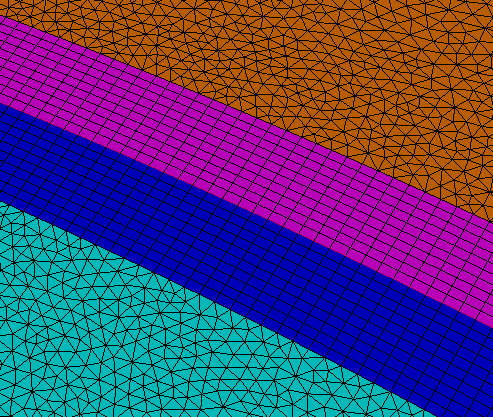
\includegraphics{figures/slidingMesh1.png}
\caption{Mesh with sliding contact boundary.}
\label{slidingmesh1}
\end{figure}

Ghosted nodes don't directly produce equations (rows) in the assembled linear system,
but can result in additional column-entries in other rows.

